\section{Amazon API Gateway}

Amazon API Gateway \cite{aws-api-gateway-docs} es un servicio que ofrece claves fundamentales que todo API Gateway debería tener: \
\begin{itemize}
	\item Único punto de entrada
	\item Conductor de Rutas
	\item Protocolo de transformación
	\item Registry and Discovery
	\item Autenticación y Autorización
	\item Escalabilidad y Orquestación
	\item Thortting (Limites)
	\item Monitorización
\end{itemize}

Pero tiene características adicionales como : \

\begin{itemize}
	\item Son basadas en HTTP
	\item Son basadas en websockets
	\item Forma parte de un set de infraestructura llamada serverless (pay as you go)
\end{itemize}
\subsection{Arquitectura}
\begin{figure}[htbp]
	\centering
	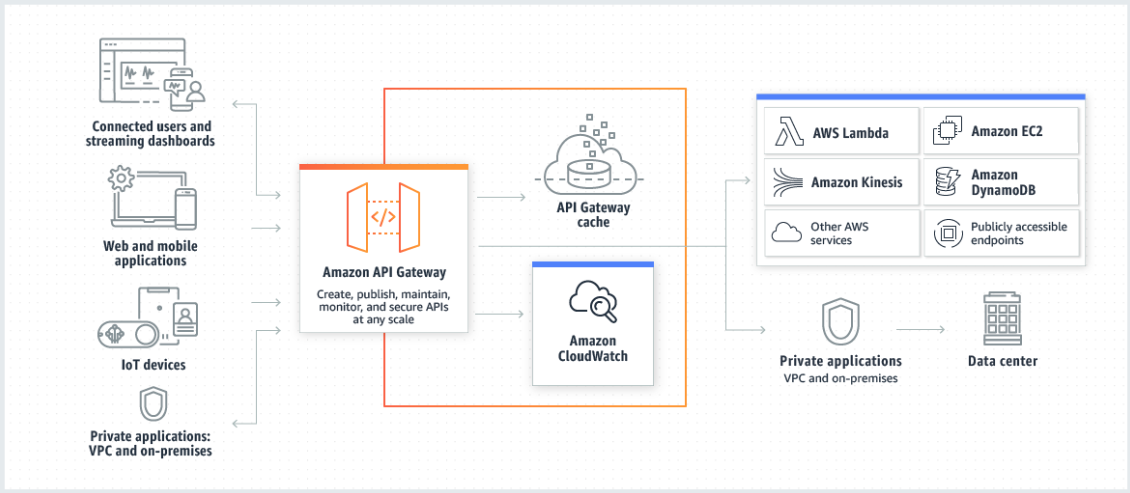
\includegraphics[width=\columnwidth]{images/architecture_aws_api_gateway}
	\caption{Arquitectura general de Aws API Gateway}
	\label{fig:architecture_aws_api_gateway}
\end{figure}

\subsection{Autenticación}
A pesar de ser un servicio de paga su autenticación es muy flexible porque te permite usar un proveedor existente de AWS tales como: AWS Identity, Access Management policies, Lambda authorizer y Amazon Cognito

\subsection{Tipos de Endpoints}
Amazon ofrece 2 tipos de Endpoints más usados:
\subsubsection{Edge Optimized API endpoints}
Las solicitudes se enrutan al Cloudfront más cercano, Point of Presence(POP). El cuál ayuda si tus clientes están distribuídos geográficamente, cuando creas un API Gateway y mantienes muchos de los parámetros por defecto no necesitas configurar esta opción ya que es el comportamiento predeterminado.

\subsubsection{Tipo de Endpoint Regional}
Especial para clientes en la misma región, por ejemplo cuando algún cliente que tiene una instancia de EC2 llama una api que también se encuentra en la misma región o también cuando necesitas baja latencia o respuesta rápida, al limitar la comunicación dentro de una región se minimiza las latencias y los costos asociados a la red.

\subsection{Integraciones}
Una vez que se define un API Method (POST, PUT, DELETE, ETC) tu necesitas definir un backend endpoint que puede ser cualquiera de:\
\begin{itemize}
	\item Ejecutar un Service Action como: SQS, STEPFUNCTION
	\item Función \textbf{Lambda}
	\item Otro \textbf{HTTP Endpoint}
\end{itemize}

Para la comunicación con el backend tu necesitas definir: \

\begin{description}
	\item[Integration Request:] Como quieres formatear la solicitud para posteriormente enviar la request formateada a tu backend
	\item[Integration Response:] Cómo quieres formatear la respuesta del backend para ser respondida al client.
\end{description}

\subsection{Validaciones}
Puedes definir validaciones antes de ejecutar tu backend, reduciendo ejecuciones innecesarias en tu backend, ya que api gateway puede retornar un error 400 al cliente sin pasar por el backend.

\subsection{Transformaciones de Data}
Te permite trasformar tu data, usando un motor de expresiones tu puedes cambiar, los headers, query arguments, body usando \textbf{mapping templates}.

\subsection{OpenApi}
Si ya tenías o usas OpenApi para definir tus endpoints puedes continuar haciendolo y agregar algunos campos adicionales para desplegar estos endpoints en API Gateway sin necesidad de definirlos de forma manual o usando IAAC.
De momento solo ofrece soporte para \textbf{OpenApi v2.0} y \textbf{OpenApi v3.0}
\subsection{Seguridad}
puedes configurar solicitudes cruzadas por endpoint (api method). También debido a que AWS tiene habilitado de forma predeterminada la detección de ataques de RED como un DOS estas siendo protegido también por toda la estructura de AWS.

\subsection{Compartir Endpoints a tus Clientes}
Puedes configurar API Keys para tus clientes y también puedes configurar También definir cuotas por API que tus clientes pueden usar así como el throttling que tus customers deben tener y si sobre pasa de estos límites Api Gateway rechazará automáticamente la solicitud.

\subsection{Monitorización}
Tienes innumerables métricas diseñadas por AWS, puedes también hacer uso de Cloudwatch logs y X-Ray. Además que en los mismos servicios puedes subscribirte a métricas y recibiendo alarmas de los eventos que 